\documentclass[conference]{IEEEtran}
\IEEEoverridecommandlockouts
\usepackage{cite}
\usepackage{amsmath,amssymb,amsfonts}
\usepackage{algorithmic}
\usepackage{graphicx}
\usepackage{textcomp}
\usepackage{xcolor}
\def\BibTeX{{\rm B\kern-.05em{\sc i\kern-.025em b}\kern-.08em
    T\kern-.1667em\lower.7ex\hbox{E}\kern-.125emX}}

\begin{document}

\title{Dynamic Graph Neural Network-Assisted Fault Diagnosis for Satellite Electrical Power Systems}

\author{
\IEEEauthorblockN{\footnotesize Dr. D. Sumathi}
\IEEEauthorblockA{\footnotesize
\textit{Dept. of Computer Science and Engineering} \\
\textit{CMR Institute of Technology} \\
Bengaluru, India \\
sumathi.d@cmrit.ac.in}
\and
\IEEEauthorblockN{\footnotesize Sanjana P Sutrave}
\IEEEauthorblockA{\footnotesize
\textit{Dept. of Computer Science and Engineering} \\
\textit{CMR Institute of Technology} \\
Bengaluru, India \\
sap23cs@cmrit.ac.in}
\and
\IEEEauthorblockN{\footnotesize R Harsha}
\IEEEauthorblockA{\footnotesize
\textit{Dept. of Computer Science and Engineering} \\
\textit{CMR Institute of Technology} \\
Bengaluru, India \\
rha23cs@cmrit.ac.in}
}

\maketitle

\begin{abstract}
\textbf{Electrical Power Systems (EPS) are critical satellite subsystems, and undetected faults
in solar arrays, batteries, or voltage regulators can directly compromise mission success.
Existing Graph Neural Network (GNN)-based fault diagnosis methods model subsystem
interactions using a fixed adjacency matrix, but this static topology cannot capture how
component importance shifts as a satellite moves between eclipse and sunlit orbital phases.
To address this limitation, we propose a Dynamic Graph Neural Network (Dynamic-GNN) that
learns a time-varying adjacency matrix $A(t)$ directly from telemetry at every timestep, rather
than assuming a fixed power-flow topology. The EPS is modeled as a 5-node graph (solar array,
battery, regulator, bus, load), combining a learned graph-attention scorer with GCN and GAT
layers and a GRU for temporal fusion, trained on 1,500 physics-simulated orbital telemetry
samples across five fault classes. Unlike static-graph approaches, the proposed model
adaptively reweights inter-component dependencies as orbital conditions change, resolving
fault signatures that fixed-topology and non-graph baselines confuse with nominal operation.
The proposed Dynamic-GNN achieves 97.3\% accuracy, 97.4\% F1-score, and a 0.996 AUC-ROC on
held-out test data, outperforming a static-graph GNN baseline (81.3\%), LSTM (82.7\%), and CNN
(76.0\%).}
\end{abstract}

\begin{IEEEkeywords}
\textbf{Satellite Electrical Power System (EPS), Fault Diagnosis, Graph Neural Network (GNN), Dynamic Graph Learning, Graph Attention Network (GAT)}
\end{IEEEkeywords}

\section{Introduction}

Electrical Power Systems (EPS) generate, store, regulate, and distribute power aboard a
satellite, and every other subsystem---from attitude control to payload instruments---depends
on a stable, well-diagnosed EPS to function. An EPS typically comprises a solar array (SA) for
power generation, a battery (BAT) for energy storage during eclipse, a power conditioning unit
(PCU) for voltage regulation and charge/discharge management, a power distribution bus (BUS),
and the aggregate spacecraft load (LOAD). Because ground engineers cannot physically inspect a
satellite in orbit, fault diagnosis must be performed entirely from downlinked telemetry, making automated,
telemetry-based fault diagnosis a critical capability for mission safety and longevity.

Recent work has applied Graph Neural Networks (GNNs) to fault diagnosis by representing a
system's components as graph nodes and their physical or data-flow relationships as edges,
capturing inter-component dependencies that convolutional or recurrent models cannot
\cite{bdi,b1,b2,b3}. As detailed in Section~\ref{sec:related}, the closest prior work---an
interpretable satellite power-system anomaly detector~\cite{bdi} and a satellite ACS fault
classifier reaching 93.4\% accuracy~\cite{b1}---and other GNN-based fault diagnosis approaches
\cite{b4,b5,b6} all construct the graph adjacency matrix once and hold it fixed for the entire
diagnosis process. This static-topology assumption cannot represent how the relative
importance of components changes with operating conditions---a satellite's EPS depends almost
entirely on the battery during eclipse and almost entirely on the solar array in sunlight, a
shift a fixed adjacency matrix has no mechanism to express.

This paper addresses this limitation for satellite EPS fault diagnosis. Specifically, this
work aims to (i) construct a physically grounded simulation of a satellite EPS capable of
generating labeled multivariate telemetry under both nominal and faulty operation, (ii) design
a GNN-based diagnosis model whose graph structure is not fixed but learned from the telemetry
itself at every timestep, and (iii) quantitatively establish, under identical training
conditions, whether such a dynamic graph improves diagnostic accuracy over a fixed-topology
GNN and over non-graph deep learning baselines. The novelty of the proposed Dynamic Graph
Neural Network (Dynamic-GNN) lies in replacing the fixed adjacency matrix used by prior
GNN-based fault diagnosis methods \cite{b1,b4,b6} with a dynamic adjacency matrix $A(t)$,
computed at every timestep from a small learned attention scorer over the current node
embeddings, and propagated through a GCN and GAT before temporal fusion with a Gated Recurrent
Unit (GRU). Unlike prior dynamic-graph work applied to time-series forecasting or industrial
process monitoring \cite{b13}, the proposed model is, to the best of our knowledge,
the first to apply timestep-wise dynamic graph construction specifically to satellite EPS
fault diagnosis, directly addressing a limitation the closest prior satellite-domain work
explicitly leaves as future work.

Section~\ref{sec:related} reviews related work; Section~\ref{sec:method} details the proposed
simulation, dataset, and architecture; Section~\ref{sec:setup} describes the experimental
setup; Section~\ref{sec:results} presents results; Section~\ref{sec:conclusion} concludes.

\section{Related Works}
\label{sec:related}

Satellite telemetry anomaly detection has been studied with both non-graph and graph-based
deep learning. Closest to the present work, Di et al.~\cite{bdi} propose an interpretable GNN
for satellite power-system anomaly detection using an adaptive graph filter, explicitly
targeting robustness to noisy and missing telemetry---but the authors state that ``the
inter-coupling relationship among the sensors of the power system remains unchanged over
time'' and accordingly hold their graph fixed after a single eigendecomposition, and their
task is binary anomaly detection rather than multi-class diagnosis, which is the gap this
paper addresses. Xu et al.~\cite{b4} and Zhao et al.~\cite{b5} instead use non-graph models
(EEMD-SVM and a Cross Attention Transformer respectively) for satellite telemetry anomaly
detection. Xie et al.~\cite{b2} and Yu et al.~\cite{b3} do apply GNNs to satellite
power-system/spacecraft telemetry with dynamic thresholding and attention-graph fusion
respectively, but both construct their graph once from feature correlations and hold it fixed
thereafter.

Beyond satellites, GNNs have been used for fault diagnosis in terrestrial power and industrial
systems, uniformly with a fixed graph: Nguyen et al.~\cite{b6} use spatial-temporal recurrent
GNNs derived from the fixed physical wiring of a power distribution network, and Wang
et al.~\cite{b7} improve robustness against non-causal shortcut features via a
causal-trivial-attention framework, without changing the underlying (fixed) topology. A
broader survey of GNN-based fault diagnosis confirms this pattern holds across essentially all
$k$-NN, prior-knowledge, and matrix-completion graph-construction methods alike~\cite{b10}.
Outside fault
diagnosis proper, graph-based learning has proven similarly effective for structured
diagnostic classification more broadly---e.g., Sumathi et al.~\cite{b20} apply a Graph
Isomorphism Network to leaf-vein structure for plant disease classification---supporting the
broader premise that representing interacting components as a graph, rather than as
independent feature vectors, better captures the structural relationships a diagnostic model
must exploit.

Dynamic graph neural networks have separately emerged as their own subfield, with time-varying
adjacency estimation flagged as a key open direction. Within time series specifically,
Zheng et al.~\cite{b13} (CST-GL) and Jin et al.~\cite{b14} (MTGODE) learn a graph structure
rather than assuming it fixed, and Pozdnyakov et al.~\cite{b15} show learned adjacency
matrices outperform fixed ones for fault diagnosis on the Tennessee Eastman Process. Outside
time series, Kavya and Sumathi~\cite{b21} fuse multimodal features over a temporally evolving
graph for
phishing-website detection, reinforcing---in a different application domain---the same
premise motivating this paper: that a fixed graph snapshot cannot capture relationships that
change with evolving behavior, and that structure should instead be recomputed as the
underlying state evolves. None of
\cite{b13,b14,b15,b21}, however, target a satellite subsystem, and \cite{b13,b14}
learn a graph once per dataset or window rather than recomputing it at every timestep as the
operating regime (e.g., eclipse vs.\ sunlit) changes \emph{within} an episode. Kumar
et al.~\cite{b18} additionally confirm LSTM remains a strong non-graph baseline for
power-system fault detection, the comparison this paper makes directly in
Section~\ref{sec:results}.

In summary, prior satellite EPS/ACS work \cite{bdi,b1} builds its graph once and holds it
fixed, while prior dynamic-graph work \cite{b13,b14,b15} targets forecasting or terrestrial
monitoring, not satellite fault diagnosis. This paper combines both directions: it extends the
satellite EPS focus of \cite{bdi} to multi-class fault diagnosis, applies timestep-wise dynamic
graph construction in the style of \cite{b13,b14,b15}, and evaluates the result against a
same-architecture fixed-graph ablation (reproducing \cite{b1,b6} adapted to the EPS) plus
non-graph CNN/LSTM baselines, isolating the contribution of dynamic graph structure
specifically.

\section{Proposed Methodology}
\label{sec:method}

The proposed system simulates a satellite EPS using physically grounded governing equations,
injects one of four fault types (or none) at a random point in a simulated orbit, and trains a
Dynamic Graph Neural Network to classify the resulting telemetry into one of five classes.
Unlike the fixed-topology graph used in prior GNN-based fault diagnosis \cite{b1,b6}, the
proposed model recomputes its adjacency matrix at every timestep from the current node
telemetry via a learned attention scorer, before propagating this dynamic graph through GCN
and GAT layers and fusing the resulting sequence with a GRU. Fig.~\ref{fig:arch} shows the
overall architecture, organized into four modules: (A) EPS simulation and dataset, (B) dynamic
graph construction, (C) the classification architecture, and (D) training and optimization.

\begin{figure}[htbp]
\centering
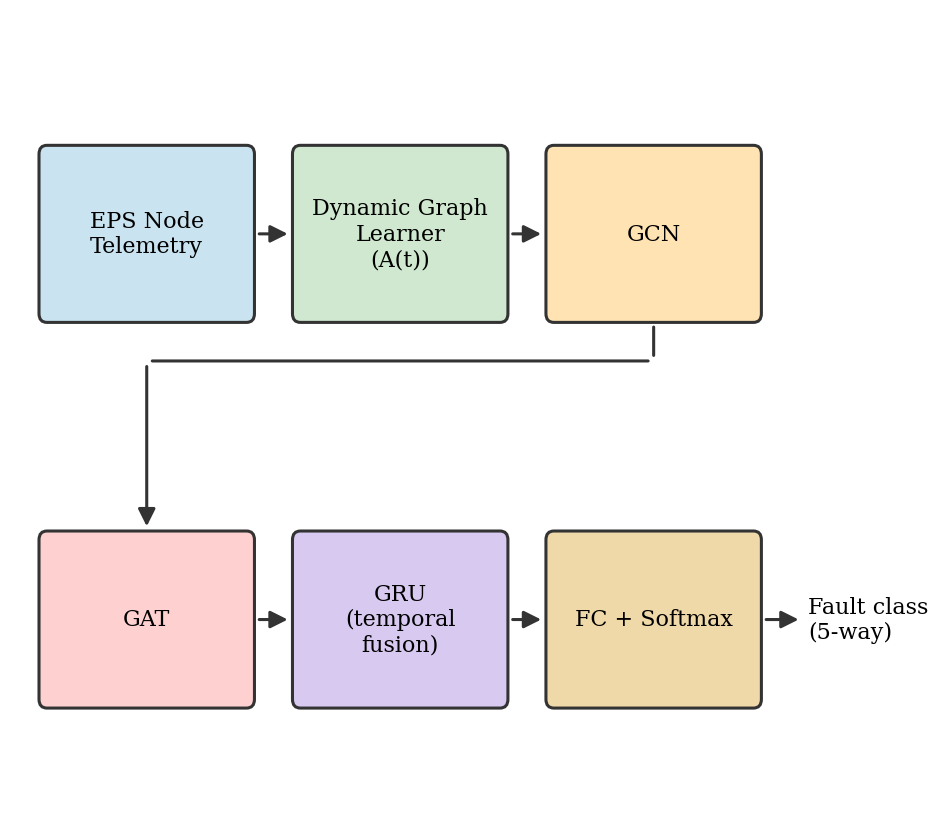
\includegraphics[width=\columnwidth]{figs/fig1_architecture.png}
\caption{Dynamic-GNN architecture.}
\label{fig:arch}
\end{figure}

\subsection{EPS Simulation and Dataset}

The satellite EPS is modeled as a directed graph $G=(V,E)$ with five nodes
$V=\{\text{SA},\text{BAT},\text{PCU},\text{BUS},\text{LOAD}\}$ representing the solar array,
battery, power conditioning unit, distribution bus, and aggregate load, connected by the
physical power-flow edges SA$\rightarrow$PCU, PCU$\rightarrow$BAT (charge),
BAT$\rightarrow$PCU (discharge), PCU$\rightarrow$BUS, BUS$\rightarrow$LOAD, and a
BUS$\rightarrow$PCU voltage-regulation feedback edge, shown in Fig.~\ref{fig:topology}. This
fixed topology is used only by the static-graph baseline (Section~\ref{sec:setup}); the
proposed model learns its own graph and does not use Fig.~\ref{fig:topology} as an input.

\begin{figure}[b]
\centering
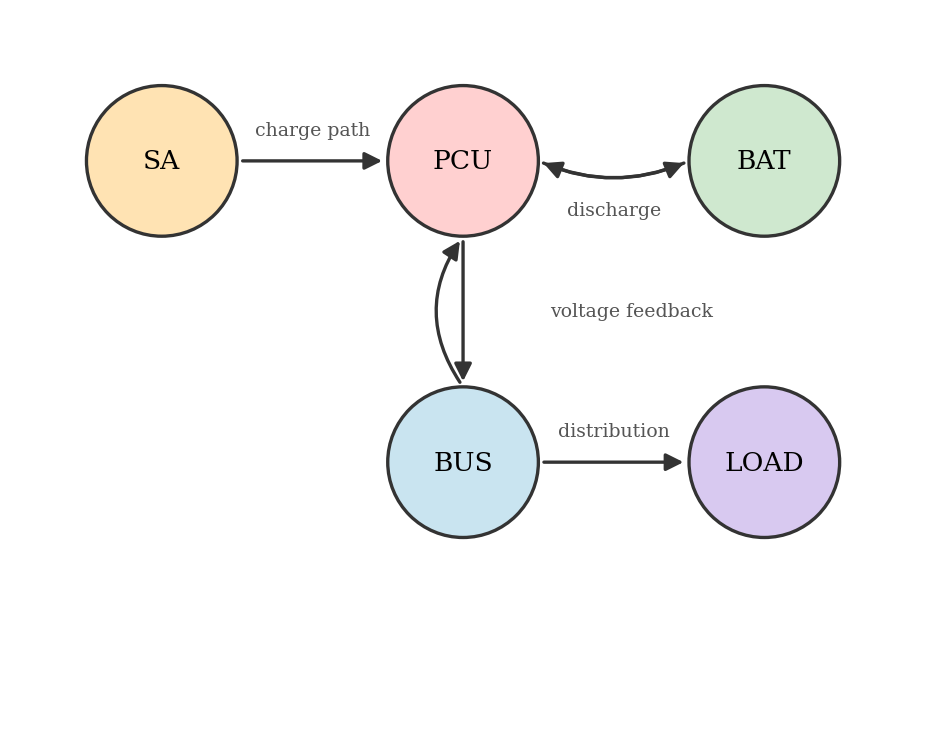
\includegraphics[width=\columnwidth]{figs/fig2_topology.png}
\caption{Fixed EPS topology (static baseline).}
\label{fig:topology}
\end{figure}

Solar array output power follows
\begin{equation}
P_{sa} = P_{max} \cdot \cos(\theta) \cdot (1 - k_d t), \quad \text{zeroed during eclipse}
\label{eq:solar}
\end{equation}
where $P_{max}$ is the beginning-of-life rated power, $\theta$ is the sun-incidence angle, and
$k_d$ is a slow panel-degradation rate. Battery state of charge evolves as
\begin{equation}
\frac{d\,SOC}{dt} = \frac{P_{charge,eff} - P_{discharge} - P_{extra}}{E_{bat}} - k_{sd} \cdot SOC
\label{eq:soc}
\end{equation}
where $E_{bat}$ is the battery's energy capacity, $P_{charge,eff}$ and $P_{discharge}$ are the
effective charge and discharge power respectively, $P_{extra}$ is a fault-injected extra drain
(zero under nominal operation), and $k_{sd}$ is a self-discharge rate. Bus voltage is
regulated as
\begin{equation}
V_{bus} = V_{nom} - k\cdot(P_{load} - P_{source}), \quad \text{clipped to regulator limits}
\label{eq:vbus}
\end{equation}
where $k$ is a droop gain and the mismatch between commanded load and available source power
determines the deviation from the nominal setpoint $V_{nom}$. At every timestep, the
source/battery power split is solved so that the physical power-balance constraint
\begin{equation}
P_{sa} + P_{bat,out} = P_{bus,load} + P_{losses}
\label{eq:balance}
\end{equation}
holds, with any solar power in excess of load and charge needs dumped by a shunt regulator,
consistent with standard EPS design practice.

One simulated episode covers one full low-Earth orbit (5760~s), sampled every 24~s into 240
timesteps, guaranteeing every episode contains a complete eclipse-to-sunlit transition. Four
fault types are injected, each at a random onset and duration within the episode:
\texttt{sa\_degradation} (a step or gradual drop in $P_{max}$ and/or incidence response),
\texttt{battery\_over\_discharge} (an unexplained extra drain $P_{extra}$ and/or reduced
charge efficiency), \texttt{pcu\_regulator\_fault} (an artificial offset injected into
$V_{bus}$ independent of the source/load balance), and \texttt{bus\_distribution\_fault}
(erratic/dropout current between BUS and LOAD unexplained by commanded load). A fifth class,
\texttt{nominal}, injects no fault. 1,500 episodes were simulated, 300 per class, and split
stratified 70:20:10 into training (1,050), validation (300), and test (150) sets.

\subsection{Dynamic Graph Construction}

At every timestep $t$, node features $x_t \in \mathbb{R}^{N\times F}$ ($N{=}5$ nodes, $F{=}5$
features: voltage, current, power, temperature, state-of-charge) are encoded by a two-layer
MLP into embeddings $h_t = \text{MLP}(x_t) \in \mathbb{R}^{N\times D}$. A dynamic adjacency
$A(t)$ is then computed via scaled dot-product scoring over these embeddings
\begin{equation}
A_{soft}(t) = \text{softmax}\!\left( \frac{h_t h_t^{\mathsf{T}}}{\sqrt{D}} \right)
\label{eq:asoft}
\end{equation}
with the diagonal excluded so that a node cannot attend to itself at this stage; a self-loop
is reintroduced during graph propagation. $A_{soft}(t)$ is a dense, continuous,
row-normalized adjacency used directly by the GCN layer. For the GAT layer, $A_{soft}(t)$ is
additionally sparsified by keeping, for each destination node, only its top-3 highest-weighted
source nodes plus a self-loop, producing a binary mask $M(t)$ that restricts attention to the
learned dynamic neighborhood while keeping the graph interpretable.

\subsection{Dynamic-GNN Classification Architecture}

Structural propagation is performed by a GCN layer
\begin{equation}
H_{gcn} = W_{gcn} \left( D(t)^{-1} (A_{soft}(t) + I)\, x_t \right)
\label{eq:gcn}
\end{equation}
where $D(t)$ is the corresponding degree diagonal matrix and $W_{gcn}$ is a learned weight
matrix. The GAT layer then computes multi-head attention restricted to $M(t)$
\begin{equation}
\alpha_{ij} = \text{softmax}_j\!\left( \text{LeakyReLU}\!\left( a_{dst}^{\mathsf{T}} h_i + a_{src}^{\mathsf{T}} h_j \right) \right), \; j \in \mathcal{N}_{M(t)}(i)
\label{eq:gat}
\end{equation}
and aggregates $h_i' = \sum_j \alpha_{ij} W_{gat} h_j$, concatenated across 2 attention heads.
The resulting per-node embeddings are mean-pooled over the 5 nodes to obtain one
32-dimensional graph-level embedding per timestep, and the resulting sequence of 240
embeddings is processed by a single-layer GRU with 80 hidden units, whose final hidden state
is passed through a dropout layer and a fully connected softmax classifier
\begin{equation}
\hat{y} = \text{softmax}(W_c h_T + b_c)
\label{eq:classifier}
\end{equation}
producing a probability distribution over the five fault classes.

\subsection{Training and Optimization}

All models are trained with the Adam optimizer (learning rate 0.001, weight decay $10^{-4}$)
to minimize the categorical cross-entropy loss
\begin{equation}
L = -\sum_i y_i \log(\hat{y}_i)
\label{eq:loss}
\end{equation}
for up to 60 epochs with early stopping (patience 10) on validation loss. For the
noise/dropout-augmented variant (Section~\ref{sec:robustness}), each training batch has a 70\%
probability of having Gaussian noise (level $\sim U(0, 0.5)\times$ per-channel standard
deviation) and/or dropout (probability $\sim U(0, 0.3)$, replacing a reading with its channel
mean) applied before the forward pass, so the model is exposed to corrupted telemetry during
training rather than only at test time.

\section{Experimental Setup}
\label{sec:setup}

All experiments were implemented in PyTorch with dense graph layers modeled after PyTorch
Geometric's API, on an Apple Silicon GPU (MPS backend). Four models were trained and compared
under identical conditions---the same 70:20:10 split, Adam settings, and a matched
18{,}000--32{,}000-parameter budget---so performance differences reflect architectural choice,
not training budget. The CNN baseline uses three 1-D convolutional layers (32/32/64 channels)
over the five nodes' features flattened into 25 channels; the LSTM baseline uses a
single-layer LSTM (48 hidden units) over the same input; the static-graph GNN uses the
identical GCN-GAT-GRU-classifier pipeline as the proposed model but with the fixed topology of
Fig.~\ref{fig:topology} substituted for the learned $A(t)$, reproducing the fixed-adjacency
principle of \cite{b1,b6} adapted to the EPS. All four models were additionally retrained with
the noise/dropout augmentation of Section~\ref{sec:method} to evaluate robustness
(Section~\ref{sec:robustness}).

\section{Results and Discussion}
\label{sec:results}

\subsection{Dataset}

The generated dataset comprises 1,500 labeled episodes, balanced at 300 per class across five
fault categories, split stratified 70:20:10. Unlike the three-class, no-nominal benchmark of
\cite{b1}, adding a nominal class makes this benchmark harder, since it and
\texttt{battery\_over\_discharge} differ only in a slow state-of-charge trend. Sanity checks
confirmed zero NaN/Inf values and that the power-balance constraint~\eqref{eq:balance} holds
to a small residual (43--45~W mean) under nominal conditions, versus a much larger residual
for \texttt{bus\_distribution\_fault} (105~W mean, 884~W max), consistent with that fault's
definition as current draw unexplained by the power balance.

\subsection{Performance Metrics}

\textbf{Accuracy}: the proportion of test episodes classified correctly,
\begin{equation}
A = \frac{TP+TN}{TP+TN+FP+FN}
\label{eq:acc}
\end{equation}

\textbf{Precision}: of the episodes predicted as a given fault class, the fraction actually
that class---a false alarm can trigger costly, unnecessary safe-mode transitions,
\begin{equation}
P = \frac{TP}{TP+FP}
\label{eq:prec}
\end{equation}

\textbf{Recall}: of the actual episodes of a given fault class, the fraction correctly
identified---arguably the more operationally dangerous failure mode, since a missed EPS
fault can propagate to loss of the spacecraft,
\begin{equation}
R = \frac{TP}{TP+FN}
\label{eq:recall}
\end{equation}

\textbf{F1-score}: the harmonic mean of precision and recall,
\begin{equation}
F1 = \frac{2PR}{P+R}
\label{eq:f1}
\end{equation}

\textbf{AUC-ROC}: the macro-averaged, one-vs-rest area under the receiver operating
characteristic curve, summarizing how well-separated each model's confidence scores are
between correct and incorrect classes across all decision thresholds, with 0.5 indicating
random guessing and 1.0 indicating perfect separation.

\textbf{Log Loss}: the categorical cross-entropy of the predicted class probabilities against
the true labels, computed as~\eqref{eq:loss}; lower log loss indicates better-calibrated
confidence, which matters because a downstream ground-operations decision may weight a
diagnosis by its reported confidence rather than treating all positive predictions equally.

\subsection{Comparative Results}

\begin{table}[htbp]
\caption{Performance Comparison of All Four Models on the Held-Out Test Set}
\begin{center}
\begin{tabular}{|l|c|c|c|c|c|c|}
\hline
\textbf{Model} & \textbf{Acc.} & \textbf{Prec.} & \textbf{Rec.} & \textbf{F1} & \textbf{AUC} & \textbf{Log} \\
 & \textbf{(\%)} & \textbf{(\%)} & \textbf{(\%)} & \textbf{(\%)} & \textbf{ROC} & \textbf{Loss} \\
\hline
CNN & 76.0 & 75.6 & 76.0 & 74.7 & 0.943 & 0.343 \\
\hline
LSTM & 82.7 & 84.3 & 82.7 & 83.1 & 0.951 & 0.432 \\
\hline
Static-GNN & 81.3 & 82.1 & 81.3 & 81.3 & 0.960 & 0.324 \\
\hline
\textbf{Dynamic-GNN} & \textbf{97.3} & \textbf{97.7} & \textbf{97.3} & \textbf{97.4} & \textbf{0.996} & \textbf{0.118} \\
\textbf{(proposed)} & & & & & & \\
\hline
\end{tabular}
\label{tab:performance}
\end{center}
\end{table}

Table~\ref{tab:performance} summarizes performance on the 150-episode held-out test set. The
proposed Dynamic-GNN outperforms all baselines across every metric, achieving \textbf{97.3\%
accuracy} (15.9--21.3 points higher than the non-graph CNN/LSTM baselines, 16.0 points higher
than the same-architecture static-graph baseline), a \textbf{0.996 AUC-ROC}, and the lowest
\textbf{log loss (0.118)}. Because the static-graph baseline shares an identical
GCN-GAT-GRU-classifier pipeline and a comparable parameter count (29{,}109 vs.\ 30{,}357),
differing only in whether the adjacency matrix is fixed or learned per timestep, this margin
isolates the contribution of dynamic graph construction specifically, not of GNNs in general.

\begin{figure}[htbp]
\centerline{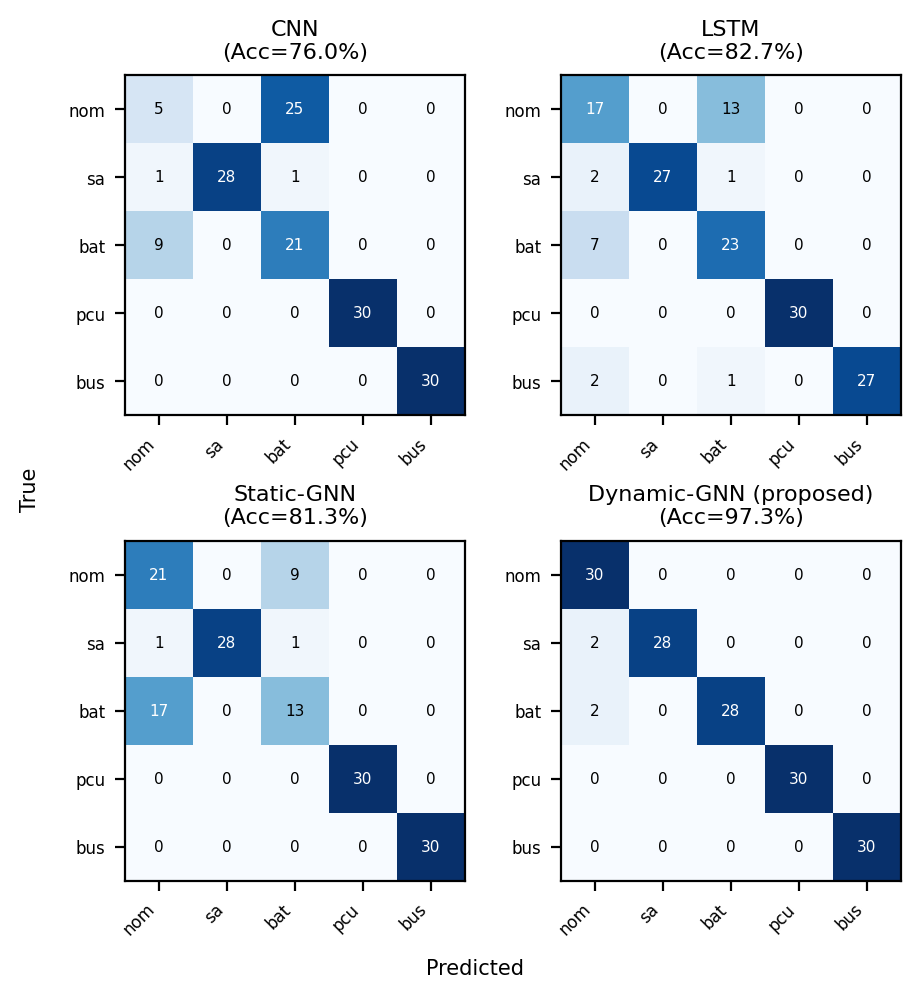
\includegraphics[width=0.95\columnwidth]{figs/fig3_confusion.png}}
\caption{Confusion matrices for all four models (test set).}
\label{fig:confusion}
\end{figure}

Fig.~\ref{fig:confusion} shows the confusion matrices for all four models. All models classify
\texttt{pcu\_regulator\_fault} and \texttt{bus\_distribution\_fault} perfectly (100\%), since
both faults produce sharp, unambiguous telemetry signatures (bus voltage railing near its
regulator limit, and erratic bus current, respectively). The dominant source of error for the
three non-dynamic models is confusion between \texttt{nominal} and
\texttt{battery\_over\_discharge}---CNN misclassifies 25 of 30 nominal test episodes as
\texttt{battery\_over\_discharge}, and the static-graph baseline confuses 9 of 30 nominal and
17 of 30 \texttt{battery\_over\_discharge} episodes---since both classes differ only in a slow
state-of-charge trend. The Dynamic-GNN reduces this specific confusion to 2 of 30 episodes in
each direction, accounting for the majority of its overall accuracy advantage.

\subsection{Interpretability Analysis}

Interpretability is essential for a diagnostic model to be trusted operationally---in a
different domain, Sumathi et al.~\cite{b22} likewise use SHAP analysis to identify which
environmental variables drive an air-quality classifier's predictions rather than treating it
as a black box, a principle applied here to the graph and attention weights instead. To verify
that the Dynamic-GNN's accuracy gain reflects physically meaningful structure rather than a
black-box artifact, GAT attention weights were analyzed per fault class and $A(t)$ was
visualized across an eclipse-to-sunlit transition.

\begin{figure}[htbp]
\centerline{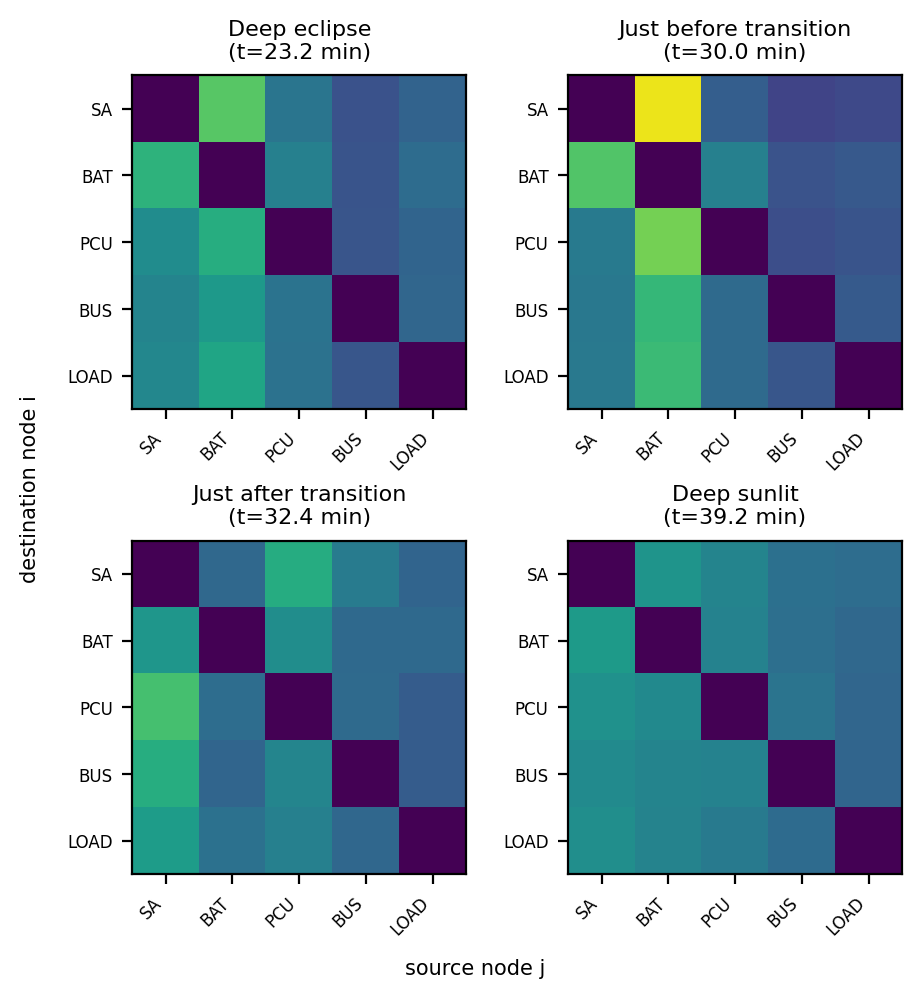
\includegraphics[width=0.95\columnwidth]{figs/fig4_adjacency.png}}
\caption{Learned adjacency $A(t)$ at four points across an eclipse$\rightarrow$sunlit transition.}
\label{fig:adjacency}
\end{figure}

Fig.~\ref{fig:adjacency} shows $A(t)$ at four points spanning one such transition: during
eclipse, the battery is the dominant source column---every other node's updated
representation depends most heavily on BAT, consistent with the battery being the only active
power source in shadow---while within approximately three timesteps ($\sim$1.2 minutes) of
the transition to sunlight, the dominant source column flips to SA, tracking the physical
handoff of power generation from battery to solar array.

\begin{figure}[htbp]
\centerline{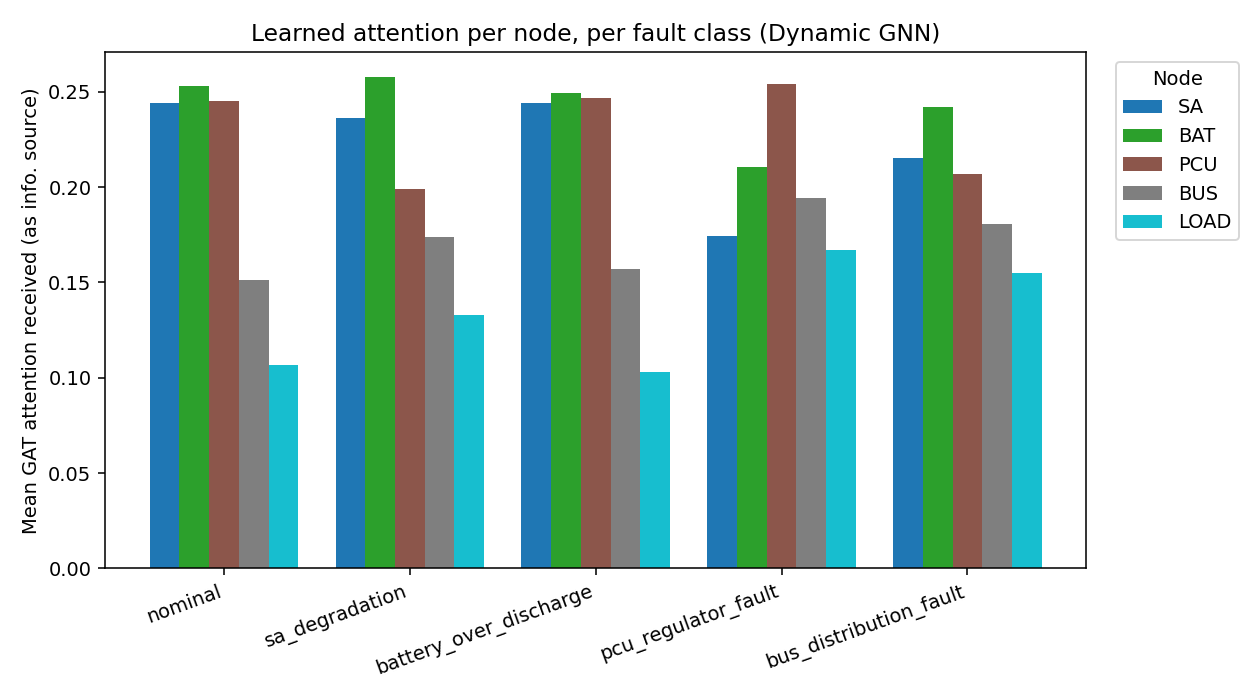
\includegraphics[width=0.95\columnwidth]{figs/fig5_attention.png}}
\caption{Mean GAT attention received per node, per fault class.}
\label{fig:attention}
\end{figure}

Fig.~\ref{fig:attention} shows mean GAT attention received per node, averaged per fault class;
while SA, BAT, and PCU receive comparable attention for \texttt{nominal},
\texttt{sa\_degradation}, and \texttt{battery\_over\_discharge} episodes, the
\texttt{pcu\_regulator\_fault} class shows a distinct shift, with PCU rising to the
most-attended node (0.254) while SA's share drops to its lowest value across all classes
(0.174), consistent with a regulator fault decoupling bus behavior from the solar array's
actual output.

We also built an interactive live demo letting a user scrub a time slider to watch $A(t)$
reconfigure in real time, shown in Fig.~\ref{fig:dashboard} just after an eclipse-to-sunlit
transition.

\begin{figure}[htbp]
\centering
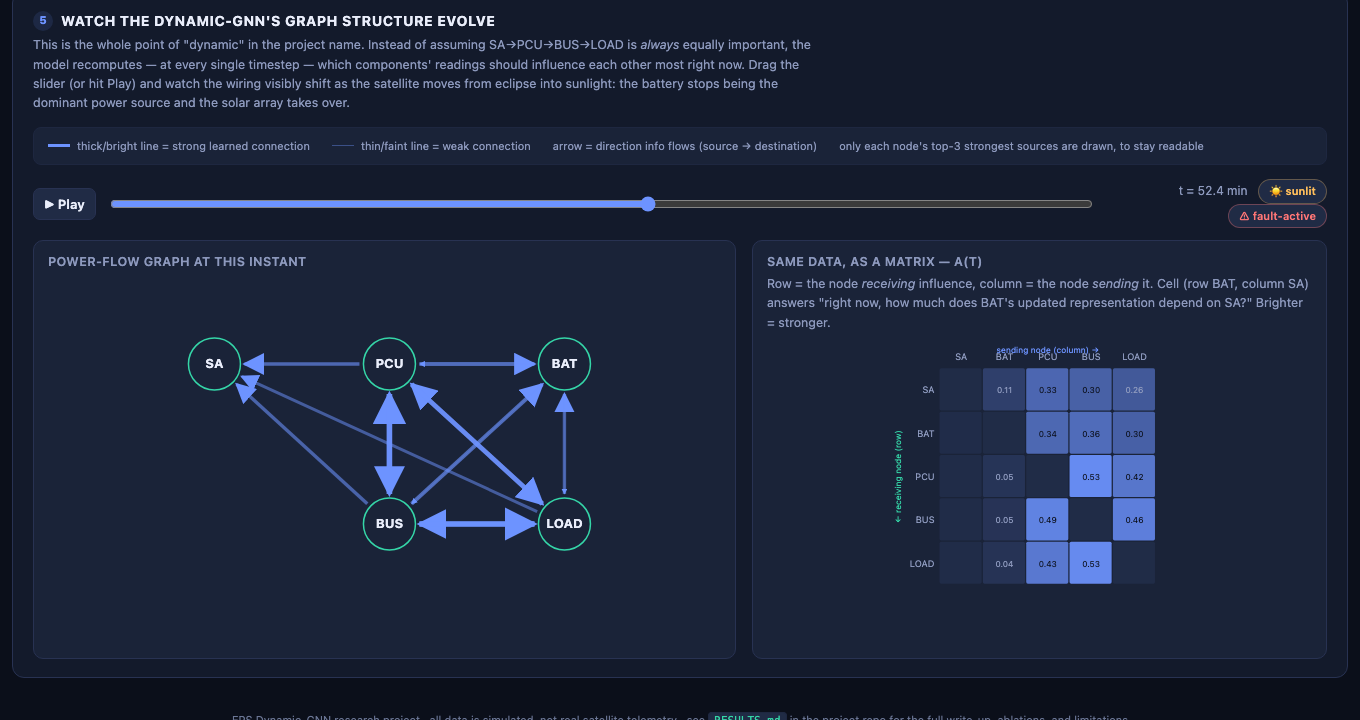
\includegraphics[width=0.80\columnwidth]{figs/fig7_dashboard.png}
\caption{Live demo: the Dynamic-GNN's learned power-flow graph and $A(t)$ matrix, scrubbable
over the orbit.}
\label{fig:dashboard}
\end{figure}

\subsection{Robustness Under Corrupted Telemetry}
\label{sec:robustness}

Following \cite{b1}'s claim of robustness to noisy and partially missing data, all four
clean-trained models were stress-tested by corrupting the test set with additive Gaussian
sensor noise (0 to $1.0\times$ the per-channel training standard deviation) and with randomly
dropped readings (0\% to 50\%, replaced with the channel mean), without retraining. The
Dynamic-GNN's advantage held or grew through moderate corruption (+11.1 points over LSTM at
$0.3\times$ noise) but collapsed sharply beyond a threshold, falling to 37.8\% accuracy at
$1.0\times$ noise, 38.7 points below the LSTM baseline at the same corruption level---likely
because the learned adjacency $A(t)$ is itself computed from the same corrupted node features,
so heavy corruption degrades both the classification and the graph structure it relies on
simultaneously.

\begin{figure}[htbp]
\centerline{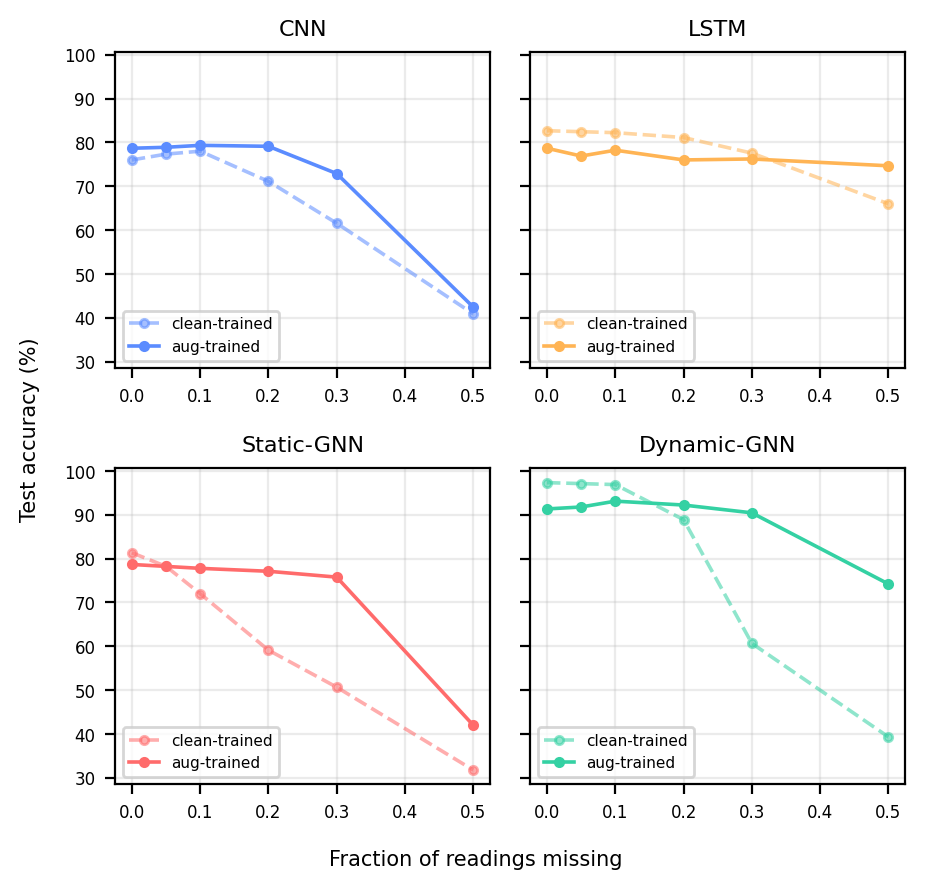
\includegraphics[width=0.78\columnwidth]{figs/fig6_robustness.png}}
\caption{Effect of noise/dropout-augmented training on missing-data robustness (dashed = clean-trained, solid = augmented-trained).}
\label{fig:robustness}
\end{figure}

Retraining all four models with noise/dropout augmentation during training
(Section~\ref{sec:method}) substantially closed this gap: the Dynamic-GNN's accuracy at 50\%
missing data rose from 39.3\% to 74.2\% (+34.9 points), shown in Fig.~\ref{fig:robustness}, at
a cost of 6.0 accuracy points on clean data (97.3\% to 91.3\%). This confirms that the dynamic
graph's clean-data advantage is real but was, before augmentation, coupled to a genuine
robustness weakness that a static or non-graph model does not share to the same degree---an
honest limitation this paper reports directly rather than omitting.

\section{Conclusion and Future Work}
\label{sec:conclusion}

This paper presented a Dynamic Graph Neural Network for satellite EPS fault diagnosis, in
which the adjacency matrix is learned from telemetry at every timestep rather than held fixed,
extending the satellite EPS anomaly-detection direction of \cite{bdi} to multi-class diagnosis
and addressing a limitation left as future work by the closest comparable satellite-domain
baseline \cite{b1}. The proposed model achieved 97.3\% accuracy, 97.4\% F1-score, and a 0.996
AUC-ROC, outperforming a same-architecture static-graph baseline (81.3\%) and non-graph CNN
(76.0\%) and LSTM (82.7\%) baselines under identical training conditions. Interpretability
analysis confirmed the learned graph tracks real physical state---the dominant power-source
column in $A(t)$ shifts from battery to solar array within minutes of the eclipse-to-sunlit
transition---and that attention shifts toward PCU specifically under regulator faults.

A robustness stress test motivated by a robustness claim in prior work revealed that the
dynamic model's advantage collapses under heavy sensor corruption, since its graph structure
depends on the same corrupted inputs it classifies; noise/dropout-augmented training
substantially, though not completely, closed this gap. Future work includes multi-seed
validation, ablations isolating the top-$k$ sparsification and attention-scorer design
choices, temporal fault localization using the per-timestep labels already collected, and
validation against real spacecraft telemetry.

\enlargethispage{110pt}
{\small
\begin{thebibliography}{00}
\bibitem{bdi} Y. Di, F. Wang, Z. Zhao, Z. Zhai, and X. Chen, ``An interpretable graph neural network for real-world satellite power system anomaly detection based on graph filtering,'' \textit{Expert Syst. Appl.}, vol. 254, p. 124348, 2024.
\bibitem{b1} Z. Wu, K. Zou, Y. Liu, and L. Zhu, ``Graph Neural Network-Assisted Fault Diagnosis for Satellite Attitude Control Systems,'' in \textit{Proc. 2025 5th Int. Conf. Electronic Information Engineering and Computer Technology (EIECT)}, 2025, pp. 580--583.
\bibitem{b2} L. Xie, D. Pi, X. Zhang, J. Chen, Y. Luo, and W. Yu, ``Graph neural network approach for anomaly detection,'' \textit{Measurement}, vol. 180, p. 109546, 2021.
\bibitem{b3} B. Yu, Y. Yu, J. Xu, G. Xiang, and Z. Yang, ``MAG: A Novel Approach for Effective Anomaly Detection in Spacecraft Telemetry Data,'' \textit{IEEE Trans. Ind. Informat.}, vol. 20, no. 3, pp. 3891--3899, 2024.
\bibitem{b4} Z. Xu, Z. Cheng, and B. Guo, ``A hybrid data-driven framework for satellite telemetry data anomaly detection,'' \textit{Acta Astronautica}, vol. 205, pp. 281--294, 2023.
\bibitem{b5} H. Zhao et al., ``Satellite Early Anomaly Detection Using an Advanced Transformer Architecture for Non-Stationary Telemetry,'' \textit{IEEE Trans. Consum. Electron.}, vol. 70, no. 1, 2024.
\bibitem{b6} B. L. H. Nguyen, T. V. Vu, T.-T. Nguyen, M. Panwar, and R. Hovsapian, ``Spatial-Temporal Recurrent Graph Neural Networks for Fault Diagnostics in Power Distribution Systems,'' \textit{IEEE Access}, vol. 11, pp. 46521--46536, 2023.
\bibitem{b7} H. Wang, R. Liu, S. X. Ding, et al., ``Causal-Trivial Attention Graph Neural Network for Fault Diagnosis of Complex Industrial Processes,'' \textit{IEEE Trans. Ind. Informat.}, vol. 20, no. 2, pp. 1489--1498, 2024.
\bibitem{b10} Z. Chen, J. Xu, C. Alippi, S. X. Ding, Y. Shardt, T. Peng, and C. Yang, ``Graph neural network-based fault diagnosis: a review,'' \textit{arXiv:2111.08185}, 2021.
\bibitem{b13} Y. Zheng, H. Y. Koh, M. Jin, L. Chi, K. T. Phan, S. Pan, Y.-P. P. Chen, and W. Xiang, ``Correlation-Aware Spatial-Temporal Graph Learning for Multivariate Time-Series Anomaly Detection,'' \textit{IEEE Trans. Neural Netw. Learn. Syst.}, 2023.
\bibitem{b14} M. Jin, Y. Zheng, Y.-F. Li, S. Chen, B. Yang, and S. Pan, ``Multivariate Time Series Forecasting With Dynamic Graph Neural ODEs,'' \textit{IEEE Trans. Knowl. Data Eng.}, vol. 35, no. 9, pp. 9168--9180, 2023.
\bibitem{b15} V. Pozdnyakov, I. Makarov, and A. Kovalenko, ``Graph Neural Networks With Trainable Adjacency Matrices for Fault Diagnosis on Multivariate Sensor Data,'' \textit{IEEE Access}, vol. 12, pp. 152860--152872, 2024.
\bibitem{b18} H. K. P. Kumar, R. K. Dash, J. R. Kalvakurthi, N. R. Atyam, and B. Mohapatra, ``High resistance fault detection in DC microgrid using Hilbert Huang transform and vector-based ensemble optimized LSTM networks,'' \textit{Sci. Rep.}, vol. 15, no. 1, Art. no. 16039, 2025.
\bibitem{b20} D. Sumathi et al., ``Early Plant Disease Detection Using Graph Isomorphic Networks: Enhancing Crop Yield Through Leaf Analysis,'' \textit{J. Comput. Sci.}, vol. 21, no. 9, pp. 2065--2073, 2025.
\bibitem{b21} S. Kavya and D. Sumathi, ``Multimodal and Temporal Graph Fusion Framework for Advanced Phishing Website Detection,'' \textit{IEEE Access}, vol. 13, pp. 74128--74146, 2025.
\bibitem{b22} D. Sumathi, S. Ayyappan, A. Sivasangari, B. Ramakrishna, P. Kanagaraju, and F. B. Kunwar, ``Random Forest with SHAP Analysis for Identifying Environmental Determinants of Air Quality in Urban Regions,'' \textit{J. Environ. Prot. Ecol.}, vol. 26, no. 8, pp. 2963--2973, 2025.
\end{thebibliography}
}

\end{document}
